% Options for packages loaded elsewhere
\PassOptionsToPackage{unicode}{hyperref}
\PassOptionsToPackage{hyphens}{url}
%
\documentclass[
  12pt,
  landscape]{article}
\usepackage{lmodern}
\usepackage{amssymb,amsmath}
\usepackage{ifxetex,ifluatex}
\ifnum 0\ifxetex 1\fi\ifluatex 1\fi=0 % if pdftex
  \usepackage[T1]{fontenc}
  \usepackage[utf8]{inputenc}
  \usepackage{textcomp} % provide euro and other symbols
\else % if luatex or xetex
  \usepackage{unicode-math}
  \defaultfontfeatures{Scale=MatchLowercase}
  \defaultfontfeatures[\rmfamily]{Ligatures=TeX,Scale=1}
\fi
% Use upquote if available, for straight quotes in verbatim environments
\IfFileExists{upquote.sty}{\usepackage{upquote}}{}
\IfFileExists{microtype.sty}{% use microtype if available
  \usepackage[]{microtype}
  \UseMicrotypeSet[protrusion]{basicmath} % disable protrusion for tt fonts
}{}
\makeatletter
\@ifundefined{KOMAClassName}{% if non-KOMA class
  \IfFileExists{parskip.sty}{%
    \usepackage{parskip}
  }{% else
    \setlength{\parindent}{0pt}
    \setlength{\parskip}{6pt plus 2pt minus 1pt}}
}{% if KOMA class
  \KOMAoptions{parskip=half}}
\makeatother
\usepackage{xcolor}
\IfFileExists{xurl.sty}{\usepackage{xurl}}{} % add URL line breaks if available
\IfFileExists{bookmark.sty}{\usepackage{bookmark}}{\usepackage{hyperref}}
\hypersetup{
  pdftitle={Assignment 5 Question 1},
  pdfauthor={Jack Ogle in collaboration with Eva Haque, Matt Lohrs, and Jack Knickrehm},
  hidelinks,
  pdfcreator={LaTeX via pandoc}}
\urlstyle{same} % disable monospaced font for URLs
\usepackage[margin=1in]{geometry}
\usepackage{color}
\usepackage{fancyvrb}
\newcommand{\VerbBar}{|}
\newcommand{\VERB}{\Verb[commandchars=\\\{\}]}
\DefineVerbatimEnvironment{Highlighting}{Verbatim}{commandchars=\\\{\}}
% Add ',fontsize=\small' for more characters per line
\usepackage{framed}
\definecolor{shadecolor}{RGB}{248,248,248}
\newenvironment{Shaded}{\begin{snugshade}}{\end{snugshade}}
\newcommand{\AlertTok}[1]{\textcolor[rgb]{0.94,0.16,0.16}{#1}}
\newcommand{\AnnotationTok}[1]{\textcolor[rgb]{0.56,0.35,0.01}{\textbf{\textit{#1}}}}
\newcommand{\AttributeTok}[1]{\textcolor[rgb]{0.77,0.63,0.00}{#1}}
\newcommand{\BaseNTok}[1]{\textcolor[rgb]{0.00,0.00,0.81}{#1}}
\newcommand{\BuiltInTok}[1]{#1}
\newcommand{\CharTok}[1]{\textcolor[rgb]{0.31,0.60,0.02}{#1}}
\newcommand{\CommentTok}[1]{\textcolor[rgb]{0.56,0.35,0.01}{\textit{#1}}}
\newcommand{\CommentVarTok}[1]{\textcolor[rgb]{0.56,0.35,0.01}{\textbf{\textit{#1}}}}
\newcommand{\ConstantTok}[1]{\textcolor[rgb]{0.00,0.00,0.00}{#1}}
\newcommand{\ControlFlowTok}[1]{\textcolor[rgb]{0.13,0.29,0.53}{\textbf{#1}}}
\newcommand{\DataTypeTok}[1]{\textcolor[rgb]{0.13,0.29,0.53}{#1}}
\newcommand{\DecValTok}[1]{\textcolor[rgb]{0.00,0.00,0.81}{#1}}
\newcommand{\DocumentationTok}[1]{\textcolor[rgb]{0.56,0.35,0.01}{\textbf{\textit{#1}}}}
\newcommand{\ErrorTok}[1]{\textcolor[rgb]{0.64,0.00,0.00}{\textbf{#1}}}
\newcommand{\ExtensionTok}[1]{#1}
\newcommand{\FloatTok}[1]{\textcolor[rgb]{0.00,0.00,0.81}{#1}}
\newcommand{\FunctionTok}[1]{\textcolor[rgb]{0.00,0.00,0.00}{#1}}
\newcommand{\ImportTok}[1]{#1}
\newcommand{\InformationTok}[1]{\textcolor[rgb]{0.56,0.35,0.01}{\textbf{\textit{#1}}}}
\newcommand{\KeywordTok}[1]{\textcolor[rgb]{0.13,0.29,0.53}{\textbf{#1}}}
\newcommand{\NormalTok}[1]{#1}
\newcommand{\OperatorTok}[1]{\textcolor[rgb]{0.81,0.36,0.00}{\textbf{#1}}}
\newcommand{\OtherTok}[1]{\textcolor[rgb]{0.56,0.35,0.01}{#1}}
\newcommand{\PreprocessorTok}[1]{\textcolor[rgb]{0.56,0.35,0.01}{\textit{#1}}}
\newcommand{\RegionMarkerTok}[1]{#1}
\newcommand{\SpecialCharTok}[1]{\textcolor[rgb]{0.00,0.00,0.00}{#1}}
\newcommand{\SpecialStringTok}[1]{\textcolor[rgb]{0.31,0.60,0.02}{#1}}
\newcommand{\StringTok}[1]{\textcolor[rgb]{0.31,0.60,0.02}{#1}}
\newcommand{\VariableTok}[1]{\textcolor[rgb]{0.00,0.00,0.00}{#1}}
\newcommand{\VerbatimStringTok}[1]{\textcolor[rgb]{0.31,0.60,0.02}{#1}}
\newcommand{\WarningTok}[1]{\textcolor[rgb]{0.56,0.35,0.01}{\textbf{\textit{#1}}}}
\usepackage{graphicx,grffile}
\makeatletter
\def\maxwidth{\ifdim\Gin@nat@width>\linewidth\linewidth\else\Gin@nat@width\fi}
\def\maxheight{\ifdim\Gin@nat@height>\textheight\textheight\else\Gin@nat@height\fi}
\makeatother
% Scale images if necessary, so that they will not overflow the page
% margins by default, and it is still possible to overwrite the defaults
% using explicit options in \includegraphics[width, height, ...]{}
\setkeys{Gin}{width=\maxwidth,height=\maxheight,keepaspectratio}
% Set default figure placement to htbp
\makeatletter
\def\fps@figure{htbp}
\makeatother
\setlength{\emergencystretch}{3em} % prevent overfull lines
\providecommand{\tightlist}{%
  \setlength{\itemsep}{0pt}\setlength{\parskip}{0pt}}
\setcounter{secnumdepth}{-\maxdimen} % remove section numbering
\usepackage{dcolumn}
\usepackage{float}

\title{Assignment 5 Question 1}
\author{Jack Ogle in collaboration with Eva Haque, Matt Lohrs, and Jack
Knickrehm}
\date{}

\begin{document}
\maketitle

\begin{enumerate}
\def\labelenumi{(\alph{enumi})}
\item
\end{enumerate}

The assumptions underlying the RDD in this paper are that in order for
the school to attain autonomy (GM) there must be a 50\% vote from the
community to have the school be GM. Clark also assumes that the school
performance, test scores, is increasing in autonomy and school effort.
Schools that are already GM at the start of a period are fully
autonomous and therefore decide only how much effort to exert. Effort in
turn improves school performance, test scores for example, but effort is
costly. Schools that are not GM at the start period must decided how
much effort to exert and whether or not to become Gm. For given effort,
non GM schools performance is assumed lower than GM school performance;
hence schools have an incentive to become GM. There are cost associated
with GM status and the decision to become one is non trivial.

The conceptual framework assumed that schools were identical. In
practice, schools differ along many dimensions, and certain types of
school may be more likely to hold and win a GM vote (e.g., those with
more entrepreneurial head teachers). Clark's empirical approach
overcomes this selection problem by focusing on the jump in performance
among schools at the 50 percent win threshold. Specifically, Clark
considers variants of the fuzzy regression discontinuity model for
school i voting on GM

\begin{enumerate}
\def\labelenumi{(\alph{enumi})}
\setcounter{enumi}{1}
\item
\end{enumerate}

These figures represent figure 8 from the paper. They are all
visualizing:

The Impact of GM Status on Schools that Become Grant-Maintained

\begin{Shaded}
\begin{Highlighting}[]
\CommentTok{# Restricting Data to (15,85) }
\NormalTok{restrict =}\StringTok{ }\KeywordTok{subset}\NormalTok{(damon, vote }\OperatorTok{<=}\StringTok{ }\DecValTok{85} \OperatorTok{&}\StringTok{ }\NormalTok{vote }\OperatorTok{>=}\StringTok{ }\DecValTok{15}\NormalTok{)}

\CommentTok{# calculating the % change}
\NormalTok{restrict}\OperatorTok{$}\NormalTok{percentage_change =}\StringTok{ }\NormalTok{restrict}\OperatorTok{$}\NormalTok{passrate2 }\OperatorTok{-}\StringTok{ }\NormalTok{restrict}\OperatorTok{$}\NormalTok{passrate0}

\CommentTok{# Base Year}
\KeywordTok{rdplot}\NormalTok{(}\DataTypeTok{y =}\NormalTok{ restrict}\OperatorTok{$}\NormalTok{passrate0, }\DataTypeTok{x =}\NormalTok{ restrict}\OperatorTok{$}\NormalTok{vote , }\DataTypeTok{c =} \DecValTok{50}\NormalTok{, }\DataTypeTok{p =} \DecValTok{3}\NormalTok{, }\DataTypeTok{nbins =} \DecValTok{7}\NormalTok{, }\DataTypeTok{title =} \StringTok{"Base Year (bin-width = 7)"}\NormalTok{, }\DataTypeTok{x.label=} \StringTok{"Vote Share"}\NormalTok{, }\DataTypeTok{y.label =} \StringTok{"% Pass"}\NormalTok{)}
\end{Highlighting}
\end{Shaded}

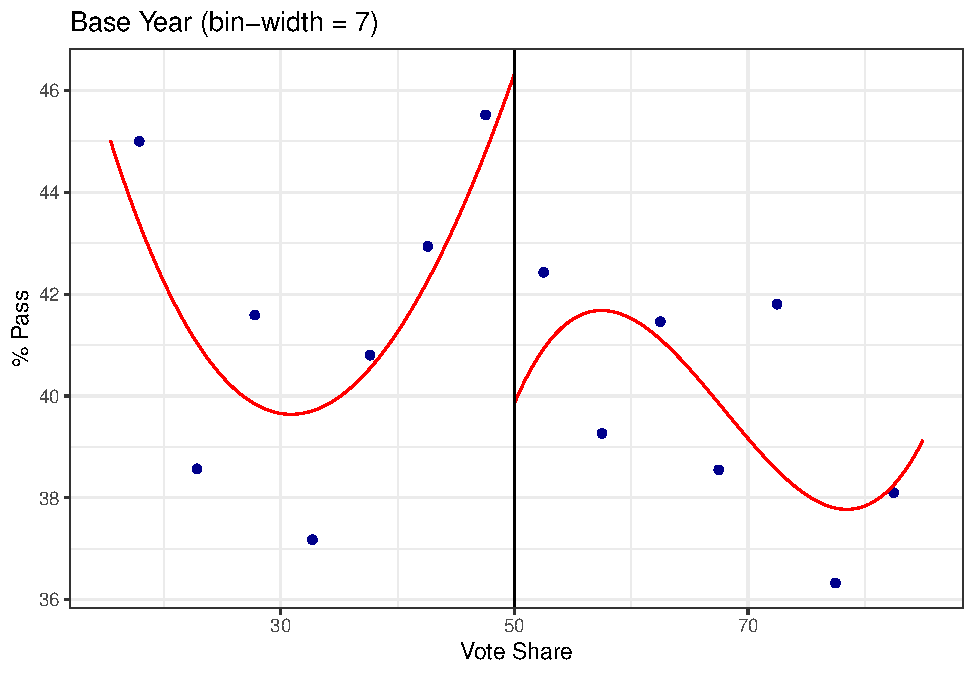
\includegraphics{Ogle_MicroMetricsAssignment_5_Q1_files/figure-latex/unnamed-chunk-2-1.pdf}

\begin{Shaded}
\begin{Highlighting}[]
\CommentTok{# Base +2 Year}
\KeywordTok{rdplot}\NormalTok{(}\DataTypeTok{y =}\NormalTok{ restrict}\OperatorTok{$}\NormalTok{passrate2, }\DataTypeTok{x =}\NormalTok{ restrict}\OperatorTok{$}\NormalTok{vote, }\DataTypeTok{c =} \DecValTok{50}\NormalTok{, }\DataTypeTok{p =} \DecValTok{3}\NormalTok{, }\DataTypeTok{nbins =} \DecValTok{7}\NormalTok{, }\DataTypeTok{title =} \StringTok{"Base + 2 Years (bin-width = 7)"}\NormalTok{, }\DataTypeTok{x.label=} \StringTok{"Vote Share"}\NormalTok{, }\DataTypeTok{y.label =} \StringTok{"% Pass"}\NormalTok{)}
\end{Highlighting}
\end{Shaded}

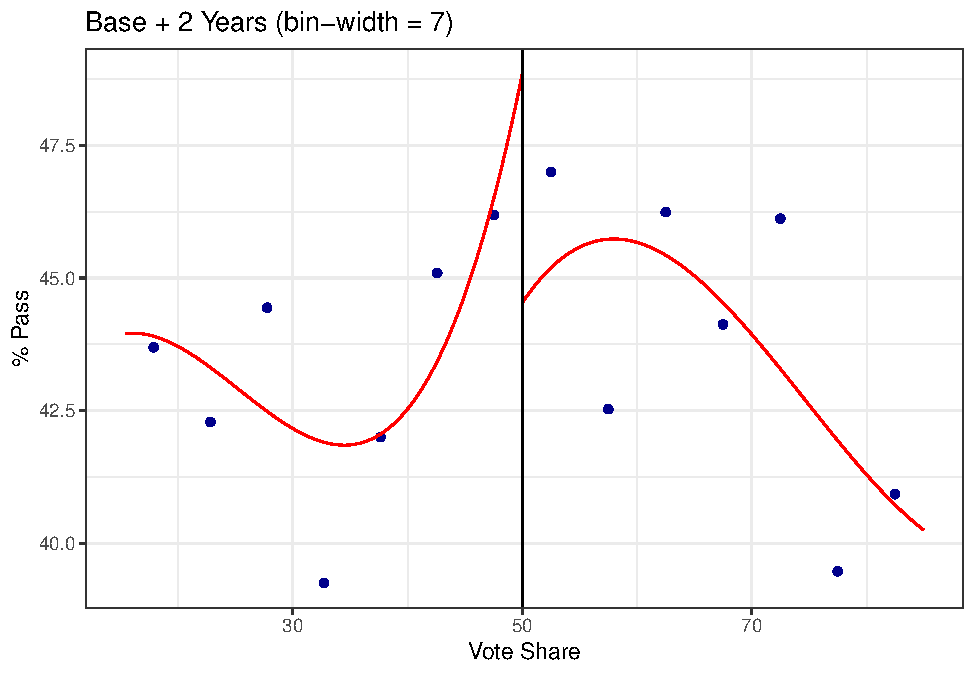
\includegraphics{Ogle_MicroMetricsAssignment_5_Q1_files/figure-latex/unnamed-chunk-2-2.pdf}

\begin{Shaded}
\begin{Highlighting}[]
\CommentTok{# % change}
\KeywordTok{rdplot}\NormalTok{(}\DataTypeTok{y =}\NormalTok{ restrict}\OperatorTok{$}\NormalTok{percentage_change, }\DataTypeTok{x =}\NormalTok{ restrict}\OperatorTok{$}\NormalTok{vote, }\DataTypeTok{p =} \DecValTok{1}\NormalTok{, }\DataTypeTok{nbins =} \DecValTok{7}\NormalTok{, }\DataTypeTok{c =} \DecValTok{50}\NormalTok{, }\DataTypeTok{title =} \StringTok{"Change (bin-width = 7)"}\NormalTok{, }\DataTypeTok{x.label=} \StringTok{"Vote Share"}\NormalTok{, }\DataTypeTok{y.label =} \StringTok{"% Pass"}\NormalTok{)}
\end{Highlighting}
\end{Shaded}

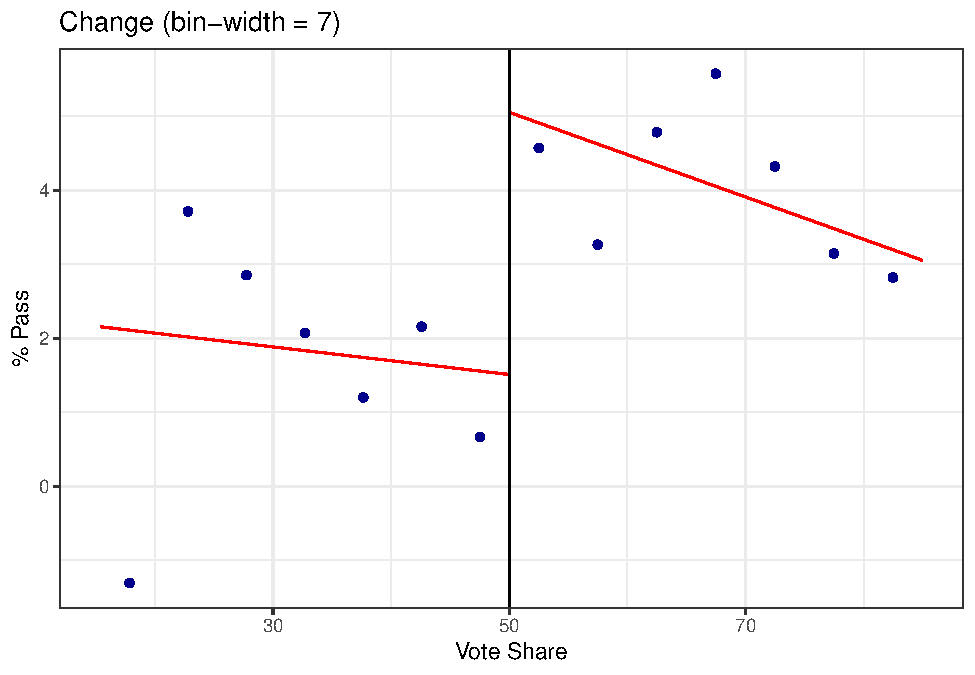
\includegraphics{Ogle_MicroMetricsAssignment_5_Q1_files/figure-latex/unnamed-chunk-2-3.pdf}

\begin{Shaded}
\begin{Highlighting}[]
\CommentTok{# Base Year}
\KeywordTok{rdplot}\NormalTok{(}\DataTypeTok{y =}\NormalTok{ restrict}\OperatorTok{$}\NormalTok{passrate0, }\DataTypeTok{x =}\NormalTok{ restrict}\OperatorTok{$}\NormalTok{vote , }\DataTypeTok{c =} \DecValTok{50}\NormalTok{, }\DataTypeTok{p =} \DecValTok{3}\NormalTok{, }\DataTypeTok{nbins =} \DecValTok{2}\NormalTok{, }\DataTypeTok{title =} \StringTok{"Base Year (bin-width = 2)"}\NormalTok{, }\DataTypeTok{x.label=} \StringTok{"Vote Share"}\NormalTok{, }\DataTypeTok{y.label =} \StringTok{"% Pass"}\NormalTok{)}
\end{Highlighting}
\end{Shaded}

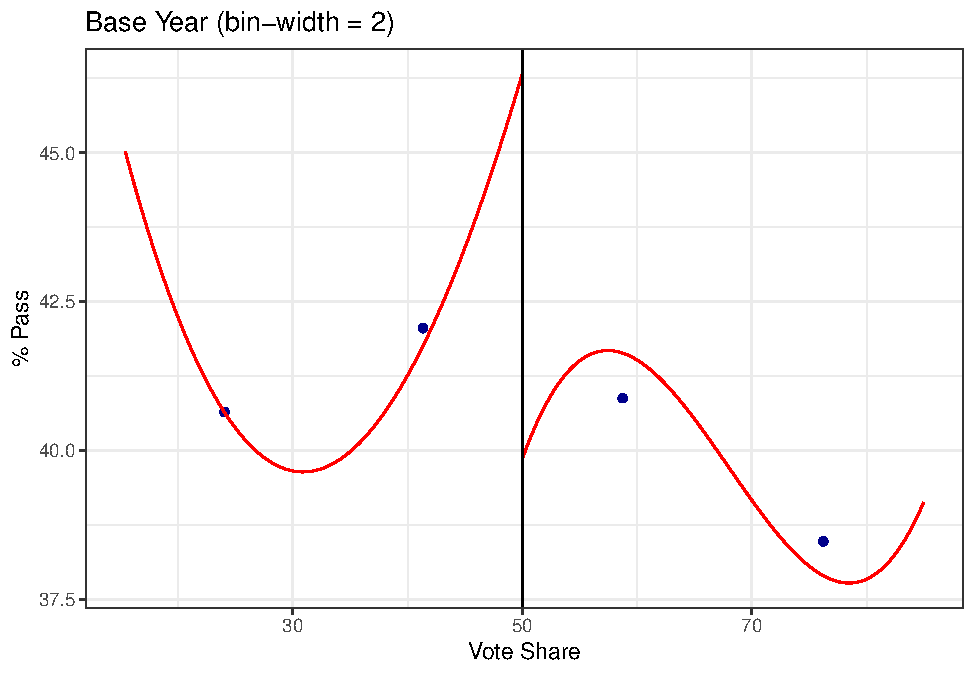
\includegraphics{Ogle_MicroMetricsAssignment_5_Q1_files/figure-latex/unnamed-chunk-2-4.pdf}

\begin{Shaded}
\begin{Highlighting}[]
\CommentTok{# Base +2 Year}
\KeywordTok{rdplot}\NormalTok{(}\DataTypeTok{y =}\NormalTok{ restrict}\OperatorTok{$}\NormalTok{passrate2, }\DataTypeTok{x =}\NormalTok{ restrict}\OperatorTok{$}\NormalTok{vote, }\DataTypeTok{c =} \DecValTok{50}\NormalTok{, }\DataTypeTok{p =} \DecValTok{3}\NormalTok{, }\DataTypeTok{nbins =} \DecValTok{2}\NormalTok{, }\DataTypeTok{title =} \StringTok{"Base + 2 Years (bin-width = 2)"}\NormalTok{, }\DataTypeTok{x.label=} \StringTok{"Vote Share"}\NormalTok{, }\DataTypeTok{y.label =} \StringTok{"% Pass"}\NormalTok{)}
\end{Highlighting}
\end{Shaded}

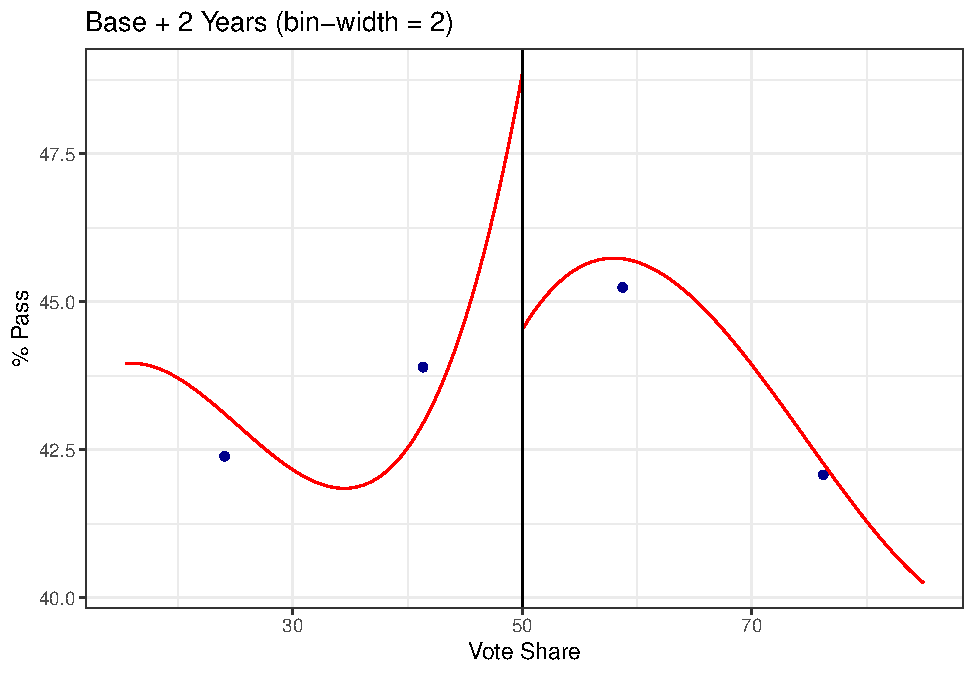
\includegraphics{Ogle_MicroMetricsAssignment_5_Q1_files/figure-latex/unnamed-chunk-2-5.pdf}

\begin{Shaded}
\begin{Highlighting}[]
\CommentTok{# % change}
\KeywordTok{rdplot}\NormalTok{(}\DataTypeTok{y =}\NormalTok{ restrict}\OperatorTok{$}\NormalTok{percentage_change, }\DataTypeTok{x =}\NormalTok{ restrict}\OperatorTok{$}\NormalTok{vote, }\DataTypeTok{p =} \DecValTok{1}\NormalTok{, }\DataTypeTok{nbins =} \DecValTok{2}\NormalTok{, }\DataTypeTok{c =} \DecValTok{50}\NormalTok{, }\DataTypeTok{title =} \StringTok{"Change (bin-width = 2)"}\NormalTok{, }\DataTypeTok{x.label=} \StringTok{"Vote Share"}\NormalTok{, }\DataTypeTok{y.label =} \StringTok{"% Pass"}\NormalTok{)}
\end{Highlighting}
\end{Shaded}

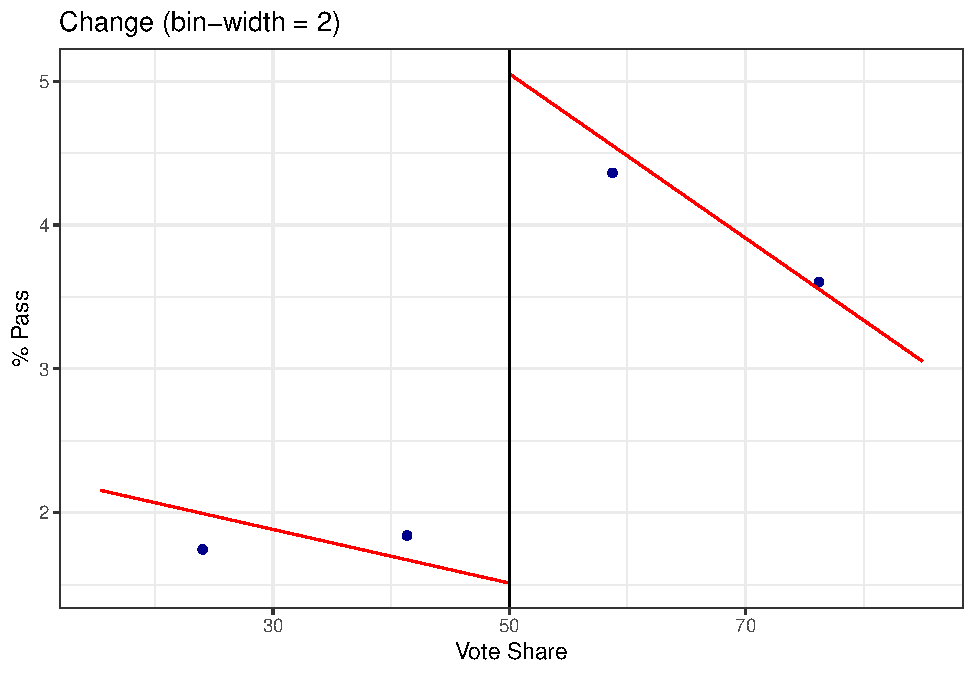
\includegraphics{Ogle_MicroMetricsAssignment_5_Q1_files/figure-latex/unnamed-chunk-2-6.pdf}

From the graphs above we can see that as you decrease the bin size from
7 which is what Clark uses in the paper for Figure 8. We can see that
there is no difference in terms of the lines of best fit, however, we
can better visualize the data with a higher bin width. We see more of
the data points.

\begin{enumerate}
\def\labelenumi{(\alph{enumi})}
\setcounter{enumi}{2}
\item
\end{enumerate}

Clark restricts his sample to those schools with votes from 15\% and
85\% because he wants to reduce bias from outliers from schools who were
very opposed or very for autonomy. For example schools with high vote
shares may have been under threat of closure, whilst few schools
received very low vote shares. Additionally, RD necessitates that in
order to estimate the average effect of a treatment you look at an
arbitrary cutoff and evaluate the treatment effects before and after the
cutoff. Additionally they saw that schools outside this interval have
different baseline characteristics and are less likely to survive. Clark
needs to estimate around the cutoff, 50, which is inside the (15,85)
interval. Other columns have functions of vote share because vote share
is the forcing variable in this Fuzzy Regression Discontinuity model.
Fuzzy RD exploits discontinuities in the probability of treatment
conditional on a variate. The discontinuity, here is Vote share, and it
becomes the IV for the treatment status. Which is why Table 3a includes
functions of vote share both on their own and interacted with the
win/lose variable.

\begin{enumerate}
\def\labelenumi{(\alph{enumi})}
\setcounter{enumi}{3}
\item
\end{enumerate}

\begin{verbatim}
## 
## % Table created by stargazer v.5.2.2 by Marek Hlavac, Harvard University. E-mail: hlavac at fas.harvard.edu
## % Date and time: Mon, Feb 21, 2022 - 09:07:34
## % Requires LaTeX packages: dcolumn 
## \begin{table}[!htbp] \centering 
##   \caption{Regression Results (d)} 
##   \label{} 
## \begin{tabular}{@{\extracolsep{5pt}}lD{.}{.}{-3} D{.}{.}{-3} D{.}{.}{-3} D{.}{.}{-3} } 
## \\[-1.8ex]\hline 
## \hline \\[-1.8ex] 
##  & \multicolumn{4}{c}{\textit{Dependent variable:}} \\ 
## \cline{2-5} 
## \\[-1.8ex] & \multicolumn{4}{c}{passrate2 - passrate0} \\ 
## \\[-1.8ex] & \multicolumn{1}{c}{(1)} & \multicolumn{1}{c}{(2)} & \multicolumn{1}{c}{(3)} & \multicolumn{1}{c}{(4)}\\ 
## \hline \\[-1.8ex] 
##  win & 2.091^{***} & 3.716^{***} & 3.542^{***} & 2.654 \\ 
##   & (0.635) & (1.283) & (1.320) & (2.015) \\ 
##   & & & & \\ 
##  margin &  & -0.045 &  &  \\ 
##   &  & (0.031) &  &  \\ 
##   & & & & \\ 
##  win\_margin &  &  & -0.057 & 0.191 \\ 
##   &  &  & (0.037) & (0.155) \\ 
##   & & & & \\ 
##  lose\_margin &  &  & -0.019 & -0.135 \\ 
##   &  &  & (0.056) & (0.220) \\ 
##   & & & & \\ 
##  win\_margin\_squared &  &  &  & -0.007^{*} \\ 
##   &  &  &  & (0.004) \\ 
##   & & & & \\ 
##  lose\_margin\_squared &  &  &  & -0.004 \\ 
##   &  &  &  & (0.007) \\ 
##   & & & & \\ 
##  Constant & 1.800^{***} & 1.096 & 1.510 & 0.853 \\ 
##   & (0.503) & (0.697) & (1.007) & (1.567) \\ 
##   & & & & \\ 
## \hline \\[-1.8ex] 
## Observations & \multicolumn{1}{c}{524} & \multicolumn{1}{c}{524} & \multicolumn{1}{c}{524} & \multicolumn{1}{c}{524} \\ 
## R$^{2}$ & \multicolumn{1}{c}{0.020} & \multicolumn{1}{c}{0.024} & \multicolumn{1}{c}{0.025} & \multicolumn{1}{c}{0.031} \\ 
## Adjusted R$^{2}$ & \multicolumn{1}{c}{0.018} & \multicolumn{1}{c}{0.021} & \multicolumn{1}{c}{0.019} & \multicolumn{1}{c}{0.021} \\ 
## Residual Std. Error & \multicolumn{1}{c}{7.025 (df = 522)} & \multicolumn{1}{c}{7.018 (df = 521)} & \multicolumn{1}{c}{7.022 (df = 520)} & \multicolumn{1}{c}{7.015 (df = 518)} \\ 
## F Statistic & \multicolumn{1}{c}{10.842$^{***}$ (df = 1; 522)} & \multicolumn{1}{c}{6.494$^{***}$ (df = 2; 521)} & \multicolumn{1}{c}{4.432$^{***}$ (df = 3; 520)} & \multicolumn{1}{c}{3.270$^{***}$ (df = 5; 518)} \\ 
## \hline 
## \hline \\[-1.8ex] 
## \textit{Note:}  & \multicolumn{4}{l}{$^{*}$p$<$0.1; $^{**}$p$<$0.05; $^{***}$p$<$0.01} \\ 
##  & \multicolumn{4}{l}{Standard errors in parentheses} \\ 
## \end{tabular} 
## \end{table}
\end{verbatim}

\begin{table}[H] \centering 
  \caption{Regression Results (d)} 
  \label{} 
\begin{tabular}{@{\extracolsep{5pt}}lD{.}{.}{-3} D{.}{.}{-3} D{.}{.}{-3} D{.}{.}{-3} } 
\\[-1.8ex]\hline 
\hline \\[-1.8ex] 
 & \multicolumn{4}{c}{\textit{Dependent variable:}} \\ 
\cline{2-5} 
\\[-1.8ex] & \multicolumn{4}{c}{passrate2 - passrate0} \\ 
\\[-1.8ex] & \multicolumn{1}{c}{(1)} & \multicolumn{1}{c}{(2)} & \multicolumn{1}{c}{(3)} & \multicolumn{1}{c}{(4)}\\ 
\hline \\[-1.8ex] 
 win & 2.091^{***} & 3.716^{***} & 3.542^{***} & 2.654 \\ 
  & (0.635) & (1.283) & (1.320) & (2.015) \\ 
  & & & & \\ 
 margin &  & -0.045 &  &  \\ 
  &  & (0.031) &  &  \\ 
  & & & & \\ 
 win\_margin &  &  & -0.057 & 0.191 \\ 
  &  &  & (0.037) & (0.155) \\ 
  & & & & \\ 
 lose\_margin &  &  & -0.019 & -0.135 \\ 
  &  &  & (0.056) & (0.220) \\ 
  & & & & \\ 
 win\_margin\_squared &  &  &  & -0.007^{*} \\ 
  &  &  &  & (0.004) \\ 
  & & & & \\ 
 lose\_margin\_squared &  &  &  & -0.004 \\ 
  &  &  &  & (0.007) \\ 
  & & & & \\ 
 Constant & 1.800^{***} & 1.096 & 1.510 & 0.853 \\ 
  & (0.503) & (0.697) & (1.007) & (1.567) \\ 
  & & & & \\ 
\hline \\[-1.8ex] 
Observations & \multicolumn{1}{c}{524} & \multicolumn{1}{c}{524} & \multicolumn{1}{c}{524} & \multicolumn{1}{c}{524} \\ 
R$^{2}$ & \multicolumn{1}{c}{0.020} & \multicolumn{1}{c}{0.024} & \multicolumn{1}{c}{0.025} & \multicolumn{1}{c}{0.031} \\ 
Adjusted R$^{2}$ & \multicolumn{1}{c}{0.018} & \multicolumn{1}{c}{0.021} & \multicolumn{1}{c}{0.019} & \multicolumn{1}{c}{0.021} \\ 
Residual Std. Error & \multicolumn{1}{c}{7.025 (df = 522)} & \multicolumn{1}{c}{7.018 (df = 521)} & \multicolumn{1}{c}{7.022 (df = 520)} & \multicolumn{1}{c}{7.015 (df = 518)} \\ 
F Statistic & \multicolumn{1}{c}{10.842$^{***}$ (df = 1; 522)} & \multicolumn{1}{c}{6.494$^{***}$ (df = 2; 521)} & \multicolumn{1}{c}{4.432$^{***}$ (df = 3; 520)} & \multicolumn{1}{c}{3.270$^{***}$ (df = 5; 518)} \\ 
\hline 
\hline \\[-1.8ex] 
\textit{Note:}  & \multicolumn{4}{l}{$^{*}$p$<$0.1; $^{**}$p$<$0.05; $^{***}$p$<$0.01} \\ 
 & \multicolumn{4}{l}{Standard errors in parentheses} \\ 
\end{tabular} 
\end{table}

\begin{itemize}
\item
  I attempted to estimate the some regressions where vote was squared,
  but I got slightly different results. I attribute this to a lack of
  data. We lack the data that is required to obtain certain regression
  results. We cannot control for all the treatments and controls
  mentioned in the empirical section of the paper where it mentions the
  design behind each regression column. However, here is the design of
  all the columns:
\item
  Column 1 describes the mean improvement difference between winners and
  losers, column 2 adds a control for vote share, and column 3 interacts
  vote share with win (the specification used to generate the fitted
  lines in Figure 8). In column 4 they weight according to the size of
  the school exam-taking cohort, to give more weight to schools with
  more exam-takers (to the extent the model is correctly specified). In
  column 5 Clark uses a quadratic vote share control function and the
  estimated impact of winning falls. This is not surprising given the
  degree of concavity in the (50,85) interval (Figure 8), although a
  cubic fit would be expected to pick up this shape (and the dip to the
  left of the 50\% threshold). In the interests of parsimony, since the
  baseline levels are relatively flat and Clark have no priors regarding
  the appropriate functional form, Clark reverts to the linear
  specification. His preferred estimates are in column 6.
\item
  If RDD is internally valid there must be \({E[Y_{0i}|X_{i}]}\) and
  \({E[Y_{1i}|X_{i}]}\) are continuous in \(X_i\) at the cutoff
  \({X_0}\). Here we can see that one of our interaction terms was
  statistically significant. This means that the assumption for internal
  validity holds because if our interaction terms all had a high degree
  of statistical significance then our win variable has a different
  effect on the passrate depending on margin and vote.
\end{itemize}

\begin{enumerate}
\def\labelenumi{(\alph{enumi})}
\setcounter{enumi}{4}
\item
\end{enumerate}

\begin{Shaded}
\begin{Highlighting}[]
\CommentTok{# Sampling smaller thresholds (95, 5)}
\NormalTok{restrict =}\StringTok{ }\KeywordTok{subset}\NormalTok{(damon, vote }\OperatorTok{<=}\StringTok{ }\DecValTok{75} \OperatorTok{&}\StringTok{ }\NormalTok{vote }\OperatorTok{>=}\StringTok{ }\DecValTok{25}\NormalTok{)}

\NormalTok{model_d_}\DecValTok{1}\NormalTok{ <-}\StringTok{ }\KeywordTok{lm}\NormalTok{(passrate2}\OperatorTok{-}\NormalTok{passrate0 }\OperatorTok{~}\StringTok{ }\NormalTok{win, }\DataTypeTok{data=}\NormalTok{restrict)}
\NormalTok{model_d_}\DecValTok{2}\NormalTok{ <-}\StringTok{ }\KeywordTok{lm}\NormalTok{(passrate2}\OperatorTok{-}\NormalTok{passrate0 }\OperatorTok{~}\StringTok{ }\NormalTok{win }\OperatorTok{+}\StringTok{ }\NormalTok{margin, }\DataTypeTok{data=}\NormalTok{restrict)}
\NormalTok{model_d_}\DecValTok{3}\NormalTok{ <-}\StringTok{ }\KeywordTok{lm}\NormalTok{(passrate2}\OperatorTok{-}\NormalTok{passrate0 }\OperatorTok{~}\StringTok{ }\NormalTok{win }\OperatorTok{+}\StringTok{ }\NormalTok{win_margin }\OperatorTok{+}\StringTok{ }\NormalTok{lose_margin, }\DataTypeTok{data=}\NormalTok{restrict)}
\NormalTok{model_d_}\DecValTok{4}\NormalTok{ <-}\StringTok{ }\KeywordTok{lm}\NormalTok{(passrate2}\OperatorTok{-}\NormalTok{passrate0 }\OperatorTok{~}\StringTok{ }\NormalTok{win }\OperatorTok{+}\StringTok{ }\NormalTok{win_margin }\OperatorTok{+}\StringTok{ }\NormalTok{lose_margin }\OperatorTok{+}\StringTok{ }\NormalTok{win_margin_squared }\OperatorTok{+}\StringTok{ }\NormalTok{lose_margin_squared, }\DataTypeTok{data =}\NormalTok{ restrict)}

\KeywordTok{stargazer}\NormalTok{(model_d_}\DecValTok{1}\NormalTok{, model_d_}\DecValTok{2}\NormalTok{, model_d_}\DecValTok{3}\NormalTok{, model_d_}\DecValTok{4}\NormalTok{, }\DataTypeTok{title=}\StringTok{"Regression Results (e)"}\NormalTok{, }\DataTypeTok{align=}\OtherTok{TRUE}\NormalTok{, }\DataTypeTok{notes =} \StringTok{"Standard errors in parentheses"}\NormalTok{, }\DataTypeTok{notes.align =} \StringTok{"l"}\NormalTok{)}
\end{Highlighting}
\end{Shaded}

\begin{verbatim}
## 
## % Table created by stargazer v.5.2.2 by Marek Hlavac, Harvard University. E-mail: hlavac at fas.harvard.edu
## % Date and time: Mon, Feb 21, 2022 - 09:07:35
## % Requires LaTeX packages: dcolumn 
## \begin{table}[!htbp] \centering 
##   \caption{Regression Results (e)} 
##   \label{} 
## \begin{tabular}{@{\extracolsep{5pt}}lD{.}{.}{-3} D{.}{.}{-3} D{.}{.}{-3} D{.}{.}{-3} } 
## \\[-1.8ex]\hline 
## \hline \\[-1.8ex] 
##  & \multicolumn{4}{c}{\textit{Dependent variable:}} \\ 
## \cline{2-5} 
## \\[-1.8ex] & \multicolumn{4}{c}{passrate2 - passrate0} \\ 
## \\[-1.8ex] & \multicolumn{1}{c}{(1)} & \multicolumn{1}{c}{(2)} & \multicolumn{1}{c}{(3)} & \multicolumn{1}{c}{(4)}\\ 
## \hline \\[-1.8ex] 
##  win & 2.724^{***} & 2.799^{*} & 2.945^{*} & 2.290 \\ 
##   & (0.757) & (1.550) & (1.561) & (2.421) \\ 
##   & & & & \\ 
##  margin &  & -0.003 &  &  \\ 
##   &  & (0.052) &  &  \\ 
##   & & & & \\ 
##  win\_margin &  &  & 0.034 & 0.023 \\ 
##   &  &  & (0.068) & (0.273) \\ 
##   & & & & \\ 
##  lose\_margin &  &  & -0.053 & 0.102 \\ 
##   &  &  & (0.080) & (0.338) \\ 
##   & & & & \\ 
##  win\_margin\_squared &  &  &  & 0.0004 \\ 
##   &  &  &  & (0.010) \\ 
##   & & & & \\ 
##  lose\_margin\_squared &  &  &  & 0.006 \\ 
##   &  &  &  & (0.013) \\ 
##   & & & & \\ 
##  Constant & 1.801^{***} & 1.765^{**} & 1.131 & 1.829 \\ 
##   & (0.561) & (0.865) & (1.158) & (1.885) \\ 
##   & & & & \\ 
## \hline \\[-1.8ex] 
## Observations & \multicolumn{1}{c}{357} & \multicolumn{1}{c}{357} & \multicolumn{1}{c}{357} & \multicolumn{1}{c}{357} \\ 
## R$^{2}$ & \multicolumn{1}{c}{0.035} & \multicolumn{1}{c}{0.035} & \multicolumn{1}{c}{0.037} & \multicolumn{1}{c}{0.038} \\ 
## Adjusted R$^{2}$ & \multicolumn{1}{c}{0.032} & \multicolumn{1}{c}{0.030} & \multicolumn{1}{c}{0.029} & \multicolumn{1}{c}{0.024} \\ 
## Residual Std. Error & \multicolumn{1}{c}{7.120 (df = 355)} & \multicolumn{1}{c}{7.130 (df = 354)} & \multicolumn{1}{c}{7.133 (df = 353)} & \multicolumn{1}{c}{7.151 (df = 351)} \\ 
## F Statistic & \multicolumn{1}{c}{12.941$^{***}$ (df = 1; 355)} & \multicolumn{1}{c}{6.454$^{***}$ (df = 2; 354)} & \multicolumn{1}{c}{4.525$^{***}$ (df = 3; 353)} & \multicolumn{1}{c}{2.746$^{**}$ (df = 5; 351)} \\ 
## \hline 
## \hline \\[-1.8ex] 
## \textit{Note:}  & \multicolumn{4}{l}{$^{*}$p$<$0.1; $^{**}$p$<$0.05; $^{***}$p$<$0.01} \\ 
##  & \multicolumn{4}{l}{Standard errors in parentheses} \\ 
## \end{tabular} 
## \end{table}
\end{verbatim}

\begin{table}[H] \centering 
  \caption{Regression Results (e)} 
  \label{} 
\begin{tabular}{@{\extracolsep{5pt}}lD{.}{.}{-3} D{.}{.}{-3} D{.}{.}{-3} D{.}{.}{-3} } 
\\[-1.8ex]\hline 
\hline \\[-1.8ex] 
 & \multicolumn{4}{c}{\textit{Dependent variable:}} \\ 
\cline{2-5} 
\\[-1.8ex] & \multicolumn{4}{c}{passrate2 - passrate0} \\ 
\\[-1.8ex] & \multicolumn{1}{c}{(1)} & \multicolumn{1}{c}{(2)} & \multicolumn{1}{c}{(3)} & \multicolumn{1}{c}{(4)}\\ 
\hline \\[-1.8ex] 
 win & 2.724^{***} & 2.799^{*} & 2.945^{*} & 2.290 \\ 
  & (0.757) & (1.550) & (1.561) & (2.421) \\ 
  & & & & \\ 
 margin &  & -0.003 &  &  \\ 
  &  & (0.052) &  &  \\ 
  & & & & \\ 
 win\_margin &  &  & 0.034 & 0.023 \\ 
  &  &  & (0.068) & (0.273) \\ 
  & & & & \\ 
 lose\_margin &  &  & -0.053 & 0.102 \\ 
  &  &  & (0.080) & (0.338) \\ 
  & & & & \\ 
 win\_margin\_squared &  &  &  & 0.0004 \\ 
  &  &  &  & (0.010) \\ 
  & & & & \\ 
 lose\_margin\_squared &  &  &  & 0.006 \\ 
  &  &  &  & (0.013) \\ 
  & & & & \\ 
 Constant & 1.801^{***} & 1.765^{**} & 1.131 & 1.829 \\ 
  & (0.561) & (0.865) & (1.158) & (1.885) \\ 
  & & & & \\ 
\hline \\[-1.8ex] 
Observations & \multicolumn{1}{c}{357} & \multicolumn{1}{c}{357} & \multicolumn{1}{c}{357} & \multicolumn{1}{c}{357} \\ 
R$^{2}$ & \multicolumn{1}{c}{0.035} & \multicolumn{1}{c}{0.035} & \multicolumn{1}{c}{0.037} & \multicolumn{1}{c}{0.038} \\ 
Adjusted R$^{2}$ & \multicolumn{1}{c}{0.032} & \multicolumn{1}{c}{0.030} & \multicolumn{1}{c}{0.029} & \multicolumn{1}{c}{0.024} \\ 
Residual Std. Error & \multicolumn{1}{c}{7.120 (df = 355)} & \multicolumn{1}{c}{7.130 (df = 354)} & \multicolumn{1}{c}{7.133 (df = 353)} & \multicolumn{1}{c}{7.151 (df = 351)} \\ 
F Statistic & \multicolumn{1}{c}{12.941$^{***}$ (df = 1; 355)} & \multicolumn{1}{c}{6.454$^{***}$ (df = 2; 354)} & \multicolumn{1}{c}{4.525$^{***}$ (df = 3; 353)} & \multicolumn{1}{c}{2.746$^{**}$ (df = 5; 351)} \\ 
\hline 
\hline \\[-1.8ex] 
\textit{Note:}  & \multicolumn{4}{l}{$^{*}$p$<$0.1; $^{**}$p$<$0.05; $^{***}$p$<$0.01} \\ 
 & \multicolumn{4}{l}{Standard errors in parentheses} \\ 
\end{tabular} 
\end{table}

\begin{itemize}
\tightlist
\item
  When I experimented with a threshold of smaller {[}25,75{]} I get
  slightly different results compared to my results previously from (d)
  and they also differ from Clark's results. Here there is a tradoff
  between bias and efficiency. We have fewer estimators that are
  statistically significant because we have less observations. This
  makes our estimators less precise. But we experience less bias from
  outliers in the data when we make our threshold smaller.
\end{itemize}

\begin{enumerate}
\def\labelenumi{(\alph{enumi})}
\setcounter{enumi}{5}
\item
\end{enumerate}

\begin{Shaded}
\begin{Highlighting}[]
\NormalTok{restrict =}\StringTok{ }\KeywordTok{subset}\NormalTok{(damon, vote }\OperatorTok{<=}\StringTok{ }\DecValTok{85} \OperatorTok{&}\StringTok{ }\NormalTok{vote }\OperatorTok{>=}\StringTok{ }\DecValTok{15}\NormalTok{)}

\NormalTok{model_f_}\DecValTok{1}\NormalTok{ <-}\StringTok{ }\KeywordTok{lm}\NormalTok{(passrate0 }\OperatorTok{~}\StringTok{ }\NormalTok{win, }\DataTypeTok{data =}\NormalTok{ restrict )}

\KeywordTok{stargazer}\NormalTok{(model_f_}\DecValTok{1}\NormalTok{, }\DataTypeTok{title=}\StringTok{"Regression Results (f)"}\NormalTok{, }\DataTypeTok{align=}\OtherTok{TRUE}\NormalTok{, }\DataTypeTok{notes =} \StringTok{"Standard errors in parentheses"}\NormalTok{, }\DataTypeTok{notes.align =} \StringTok{"l"}\NormalTok{)}
\end{Highlighting}
\end{Shaded}

\begin{verbatim}
## 
## % Table created by stargazer v.5.2.2 by Marek Hlavac, Harvard University. E-mail: hlavac at fas.harvard.edu
## % Date and time: Mon, Feb 21, 2022 - 09:07:35
## % Requires LaTeX packages: dcolumn 
## \begin{table}[!htbp] \centering 
##   \caption{Regression Results (f)} 
##   \label{} 
## \begin{tabular}{@{\extracolsep{5pt}}lD{.}{.}{-3} } 
## \\[-1.8ex]\hline 
## \hline \\[-1.8ex] 
##  & \multicolumn{1}{c}{\textit{Dependent variable:}} \\ 
## \cline{2-2} 
## \\[-1.8ex] & \multicolumn{1}{c}{passrate0} \\ 
## \hline \\[-1.8ex] 
##  win & -2.082 \\ 
##   & (1.364) \\ 
##   & \\ 
##  Constant & 41.462^{***} \\ 
##   & (1.081) \\ 
##   & \\ 
## \hline \\[-1.8ex] 
## Observations & \multicolumn{1}{c}{524} \\ 
## R$^{2}$ & \multicolumn{1}{c}{0.004} \\ 
## Adjusted R$^{2}$ & \multicolumn{1}{c}{0.003} \\ 
## Residual Std. Error & \multicolumn{1}{c}{15.093 (df = 522)} \\ 
## F Statistic & \multicolumn{1}{c}{2.329 (df = 1; 522)} \\ 
## \hline 
## \hline \\[-1.8ex] 
## \textit{Note:}  & \multicolumn{1}{l}{$^{*}$p$<$0.1; $^{**}$p$<$0.05; $^{***}$p$<$0.01} \\ 
##  & \multicolumn{1}{l}{Standard errors in parentheses} \\ 
## \end{tabular} 
## \end{table}
\end{verbatim}

\begin{table}[H] \centering 
  \caption{Regression Results (f)} 
  \label{} 
\begin{tabular}{@{\extracolsep{5pt}}lD{.}{.}{-3} } 
\\[-1.8ex]\hline 
\hline \\[-1.8ex] 
 & \multicolumn{1}{c}{\textit{Dependent variable:}} \\ 
\cline{2-2} 
\\[-1.8ex] & \multicolumn{1}{c}{passrate0} \\ 
\hline \\[-1.8ex] 
 win & -2.082 \\ 
  & (1.364) \\ 
  & \\ 
 Constant & 41.462^{***} \\ 
  & (1.081) \\ 
  & \\ 
\hline \\[-1.8ex] 
Observations & \multicolumn{1}{c}{524} \\ 
R$^{2}$ & \multicolumn{1}{c}{0.004} \\ 
Adjusted R$^{2}$ & \multicolumn{1}{c}{0.003} \\ 
Residual Std. Error & \multicolumn{1}{c}{15.093 (df = 522)} \\ 
F Statistic & \multicolumn{1}{c}{2.329 (df = 1; 522)} \\ 
\hline 
\hline \\[-1.8ex] 
\textit{Note:}  & \multicolumn{1}{l}{$^{*}$p$<$0.1; $^{**}$p$<$0.05; $^{***}$p$<$0.01} \\ 
 & \multicolumn{1}{l}{Standard errors in parentheses} \\ 
\end{tabular} 
\end{table}

There is no reason to use passrate0 as the dependent variable as we want
to estimate the effect of the autonomy of schools on pass rate. The vote
would have had little to now effect on the pass rate in the base year.
The base year is important because we can regress the difference in the
base year + 2 with the base year to get a significant result. This does
not invalidate the results. The result here is that on average a school
that has one the election has a \%200 reduction in pass rate. This
result is not statistically significant and therefore does not affect
nor invalidate our RDD.

\begin{enumerate}
\def\labelenumi{(\alph{enumi})}
\setcounter{enumi}{6}
\item
\end{enumerate}

In addition to points e and f we can include further evidence about the
relationship between the variables. We can see here that there is not
much difference between the amount of observations before the 50\%
cutoff and after the cutoff. If there was a large difference then it
would invalidate our RDD because it would mean that assignment of the
treatment versus control is not as good as randomly assigned.

\begin{Shaded}
\begin{Highlighting}[]
\NormalTok{restrict =}\StringTok{ }\KeywordTok{subset}\NormalTok{(damon, vote }\OperatorTok{<=}\StringTok{ }\DecValTok{85} \OperatorTok{&}\StringTok{ }\NormalTok{vote }\OperatorTok{>=}\StringTok{ }\DecValTok{15}\NormalTok{)}
\KeywordTok{ggplot}\NormalTok{(}\DataTypeTok{data =}\NormalTok{ restrict, }\KeywordTok{aes}\NormalTok{(vote)) }\OperatorTok{+}
\StringTok{  }\KeywordTok{geom_density}\NormalTok{()}\OperatorTok{+}
\StringTok{  }\KeywordTok{labs}\NormalTok{(}\DataTypeTok{title =} \StringTok{"Density plot of Vote Share"}\NormalTok{) }\OperatorTok{+}
\StringTok{  }\KeywordTok{xlab}\NormalTok{(}\StringTok{"Vote Share"}\NormalTok{) }\OperatorTok{+}
\StringTok{  }\KeywordTok{ylab}\NormalTok{(}\StringTok{"Density"}\NormalTok{)}
\end{Highlighting}
\end{Shaded}

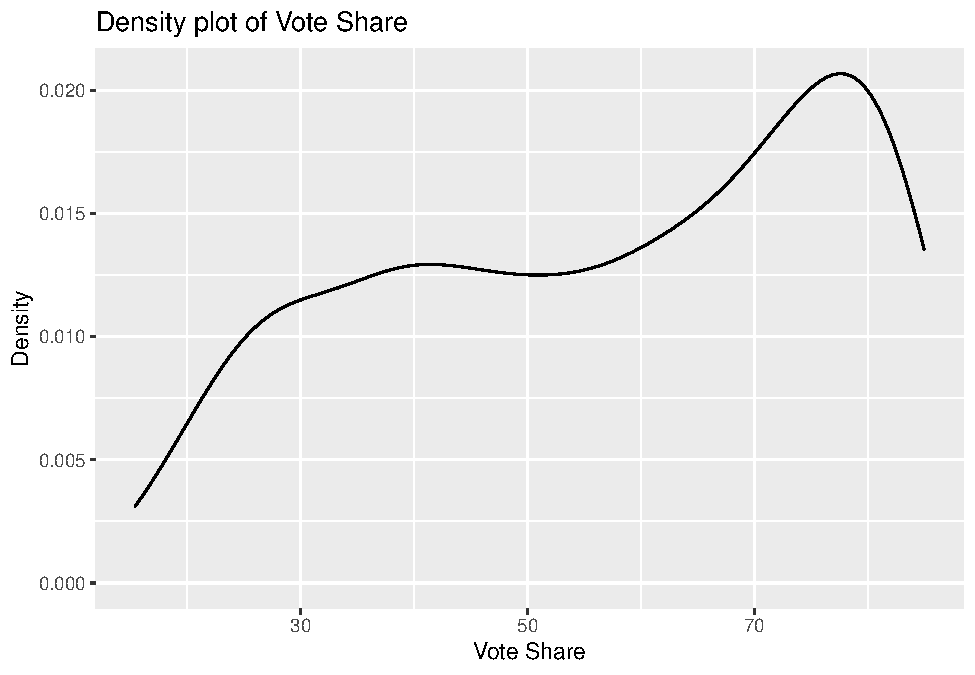
\includegraphics{Ogle_MicroMetricsAssignment_5_Q1_files/figure-latex/unnamed-chunk-6-1.pdf}

\begin{enumerate}
\def\labelenumi{(\alph{enumi})}
\setcounter{enumi}{7}
\item
\end{enumerate}

The validity of RD estimates depends crucially on the assumption that
the polynomials provide and adequate representation of E {[}Y0i
\textbar{} Xi {]} If not what looks like a jump may simply be a
non-linearity in f (Xi) that the polynomials have not accounted for. A
regression discontinuity method is close to an experiment under ideal
conditions, in reducing selection bias (high internal validity), and in
presenting challenges to broader generalization (low external validity).

\begin{enumerate}
\def\labelenumi{(\roman{enumi})}
\item
\end{enumerate}

\begin{Shaded}
\begin{Highlighting}[]
\KeywordTok{rdrobust}\NormalTok{(restrict}\OperatorTok{$}\NormalTok{passrate2}\OperatorTok{-}\NormalTok{restrict}\OperatorTok{$}\NormalTok{passrate0, restrict}\OperatorTok{$}\NormalTok{vote, }\DataTypeTok{c=}\DecValTok{50}\NormalTok{)}
\end{Highlighting}
\end{Shaded}

\begin{verbatim}
## Call: rdrobust
## 
## Number of Obs.                  524
## BW type                       mserd
## Kernel                   Triangular
## VCE method                       NN
## 
## Number of Obs.                  195          329
## Eff. Number of Obs.              59           66
## Order est. (p)                    1            1
## Order bias  (q)                   2            2
## BW est. (h)                   9.678        9.678
## BW bias (b)                  15.263       15.263
## rho (h/b)                     0.634        0.634
## Unique Obs.                     193          326
\end{verbatim}

\begin{Shaded}
\begin{Highlighting}[]
\NormalTok{restrict_rd <-}\StringTok{ }\KeywordTok{subset}\NormalTok{(restrict, vote }\OperatorTok{>}\StringTok{ }\DecValTok{50} \OperatorTok{-}\StringTok{ }\FloatTok{9.678} \OperatorTok{&}\StringTok{ }\NormalTok{vote }\OperatorTok{<}\StringTok{ }\DecValTok{50} \OperatorTok{+}\StringTok{ }\FloatTok{9.678}\NormalTok{)}

\NormalTok{model_}\DecValTok{1}\NormalTok{_i <-}\StringTok{ }\KeywordTok{lm}\NormalTok{(passrate2}\OperatorTok{-}\NormalTok{passrate0 }\OperatorTok{~}\StringTok{ }\NormalTok{win, }\DataTypeTok{data=}\NormalTok{restrict_rd)}
\KeywordTok{stargazer}\NormalTok{(model_}\DecValTok{1}\NormalTok{_i, }\DataTypeTok{title=}\StringTok{"Regression Results (f)"}\NormalTok{, }\DataTypeTok{align=}\OtherTok{TRUE}\NormalTok{, }\DataTypeTok{notes =} \StringTok{"Standard errors in parentheses"}\NormalTok{, }\DataTypeTok{notes.align =} \StringTok{"l"}\NormalTok{)}
\end{Highlighting}
\end{Shaded}

\begin{verbatim}
## 
## % Table created by stargazer v.5.2.2 by Marek Hlavac, Harvard University. E-mail: hlavac at fas.harvard.edu
## % Date and time: Mon, Feb 21, 2022 - 09:07:35
## % Requires LaTeX packages: dcolumn 
## \begin{table}[!htbp] \centering 
##   \caption{Regression Results (f)} 
##   \label{} 
## \begin{tabular}{@{\extracolsep{5pt}}lD{.}{.}{-3} } 
## \\[-1.8ex]\hline 
## \hline \\[-1.8ex] 
##  & \multicolumn{1}{c}{\textit{Dependent variable:}} \\ 
## \cline{2-2} 
## \\[-1.8ex] & \multicolumn{1}{c}{passrate2 - passrate0} \\ 
## \hline \\[-1.8ex] 
##  win & 2.571^{*} \\ 
##   & (1.367) \\ 
##   & \\ 
##  Constant & 1.475 \\ 
##   & (0.993) \\ 
##   & \\ 
## \hline \\[-1.8ex] 
## Observations & \multicolumn{1}{c}{125} \\ 
## R$^{2}$ & \multicolumn{1}{c}{0.028} \\ 
## Adjusted R$^{2}$ & \multicolumn{1}{c}{0.020} \\ 
## Residual Std. Error & \multicolumn{1}{c}{7.628 (df = 123)} \\ 
## F Statistic & \multicolumn{1}{c}{3.538$^{*}$ (df = 1; 123)} \\ 
## \hline 
## \hline \\[-1.8ex] 
## \textit{Note:}  & \multicolumn{1}{l}{$^{*}$p$<$0.1; $^{**}$p$<$0.05; $^{***}$p$<$0.01} \\ 
##  & \multicolumn{1}{l}{Standard errors in parentheses} \\ 
## \end{tabular} 
## \end{table}
\end{verbatim}

\begin{table}[!htbp] \centering 
  \caption{Regression Results (f)} 
  \label{} 
\begin{tabular}{@{\extracolsep{5pt}}lD{.}{.}{-3} } 
\\[-1.8ex]\hline 
\hline \\[-1.8ex] 
 & \multicolumn{1}{c}{\textit{Dependent variable:}} \\ 
\cline{2-2} 
\\[-1.8ex] & \multicolumn{1}{c}{passrate2 - passrate0} \\ 
\hline \\[-1.8ex] 
 win & 2.571^{*} \\ 
  & (1.367) \\ 
  & \\ 
 Constant & 1.475 \\ 
  & (0.993) \\ 
  & \\ 
\hline \\[-1.8ex] 
Observations & \multicolumn{1}{c}{125} \\ 
R$^{2}$ & \multicolumn{1}{c}{0.028} \\ 
Adjusted R$^{2}$ & \multicolumn{1}{c}{0.020} \\ 
Residual Std. Error & \multicolumn{1}{c}{7.628 (df = 123)} \\ 
F Statistic & \multicolumn{1}{c}{3.538$^{*}$ (df = 1; 123)} \\ 
\hline 
\hline \\[-1.8ex] 
\textit{Note:}  & \multicolumn{1}{l}{$^{*}$p$<$0.1; $^{**}$p$<$0.05; $^{***}$p$<$0.01} \\ 
 & \multicolumn{1}{l}{Standard errors in parentheses} \\ 
\end{tabular} 
\end{table}

\begin{enumerate}
\def\labelenumi{(\alph{enumi})}
\setcounter{enumi}{9}
\item
\end{enumerate}

I used this package for b so my results are the same. One thing that I
noticed is that when you increase the binwidth the data collapses and
you miss certain nuances in the visualization. The opposite is true when
you decrease it.

\end{document}
